\chapter{Evaluation and Results} \label{chap:Evaluation and Results}

We evaluated our algorithm by building an adhoc cluster in AWS. We
have used Mesos as our resource manager for our cluster. Our compute
cluster has one mesos master node. This also runs a spark history
server. This node is not used for any computation. This node is
primarily to monitor slave node and do resource scheduling. We have ten slave
nodes where all the computation happens. Each slave node has
8 vCPUs, 64 GB RAM and 160 GB Hard disk. The master node has 8 vCPUs,
16GB RAM and 160 GB Hard disk. Each vCPU is approximately 1/2 a
core. vCPU is unit used by AWS. All the nodes are running ubuntu as
base OS.

We performed experiments on two real datasets.
\begin{enumerate}
\item \textbf{Higgs Dataset:}
Higgs Dataset contains 28 features. These features are kinematic
properties measured by the particle detectors in the
accelerator. Classes are signal process which produces Higgs boson and
background process which does not. The dataset contains 11 Million
vectors with classes.

\item \textbf{Forest Dataset:}
Forest Dataset is a real dataset which predicts the cover type of
forest from cartographic variables. It has 6 different classes. Each
vector has 54 attributes. Out of 54 only the first 10 are integer
attributes and rest are binary. we have used only first 10 attributes
in our tests. The dataset is relatively small and contains only 580K
vectors with classes.
\end{enumerate}


Since there are no available implementation available in spark, the
only benchmark we can compare against is brute force algorithm. So we
have implemented the bruteforce algorithm in spark leveraging the
parallel computation.

In our experiments we analysed the effect of the following variables on the
overall runtime and shuffle data
\begin{enumerate}
\item Size of the dataset
\item Number of Neighbours (k)
\item Number of pivots
\item Number of compute Nodes
\item Number of dimensions
\end{enumerate}


\section{Effect of size of dataset}

We have studied the effect of size of the dataset on overall running
time. We have compared the results against bruteforce algorithm.
We have used Higgs Dataset with 6 dimensions. Below figure shows how
the running time varies when the dataset increases.

From the graph we can see that as the dataset doubles the running time
increases quadratically. Our proposed algorithm
completed the 1 Million x 1 Million self join
in 2.2 minutes where as the brute force algorithm took about 3.9
hours. We are getting approximately 100 times faster even with the small
dataset. With the larger datasets like 11 Million x 11 Million, our
algorithm completed within 26 minutes. We did not run the bruteforce
algorithm in such a large dataset as time taken will be too long. But
based on the quadratic increase we have seen, our algorithm will be in comparison with
brute force about 800 to 1000 times faster.

\bigskip

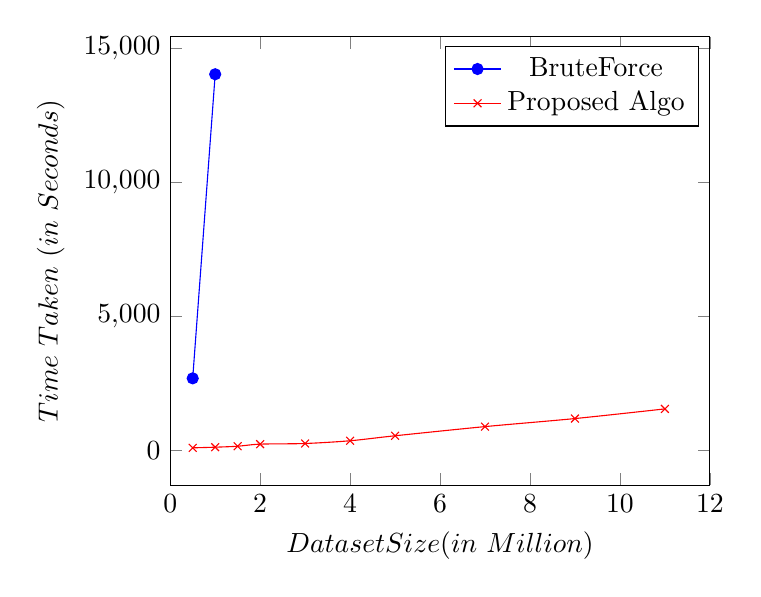
\begin{tikzpicture}[scale=1.0]
  \begin{axis}[
    xlabel=$Dataset Size(in\ Million)$,
    scaled x ticks = false,
    scaled y ticks = false,
    xmin=0, xmax=12,
    ylabel=$Time\ Taken\ (in\ Seconds)$]
    \addplot[smooth,mark=*,blue] plot coordinates {
      (0.5, 2700)
      (1, 14040)
    };
    \addlegendentry{BruteForce}

    \addplot[smooth,color=red,mark=x]
    plot coordinates {
      (0.5, 108)
      (1, 132)
      (1.500, 168)
      (2.000, 246)
      (3.000, 270)
      (4.000, 372)
      (5.000, 558)
      (7.000, 900)
      (9.000, 1200)
      (11.000, 1560)
    };
    \addlegendentry{Proposed Algo}
  \end{axis}
\end{tikzpicture}

\section{Effect of k}

Here we have evaluated the effect of number of neighbour calculation
on the total time taken. Since the performance of bruteforce is very low, we will not using the
comparison chart anymore. Here we have used the Higgs dataset with
500k vectors. The time taken increases linearly with increase in k. We
also see that the number of shuffle bytes as well increase with
increase in k. This is because with increase in k, we need to find
more k across partitions.

\medskip

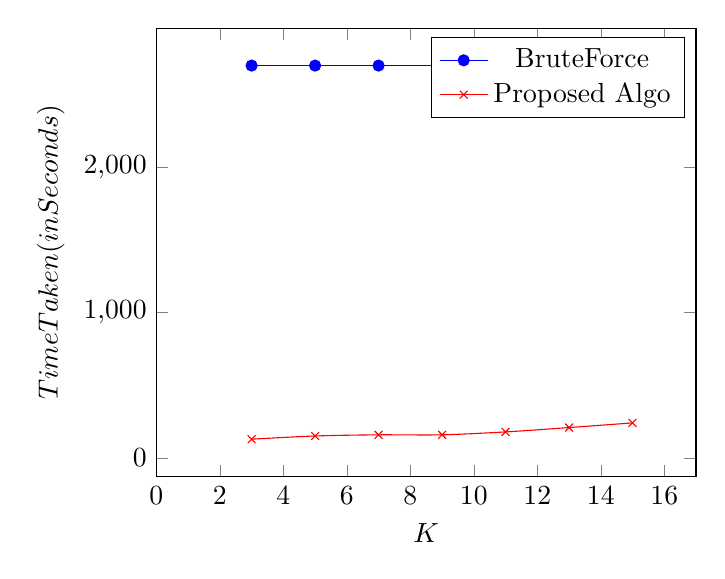
\begin{tikzpicture}[scale=1.0]
  \begin{axis}[
    xlabel=$K$,
    scaled x ticks = false,
    scaled y ticks = false,
    xmin=0, xmax=17,
    ylabel=$TimeTaken(inSeconds)$]
    \addplot[smooth,mark=*,blue] plot coordinates {
      (3, 2700)
      (5, 2700)
      (7, 2700)
      (9, 2700)
      (11, 2700)
      (13, 2700)
      (15, 2700)
    };
    \addlegendentry{BruteForce}

    \addplot[smooth,color=red,mark=x]
    plot coordinates {
      (3, 130)
      (5, 152)
      (7, 160)
      (9, 160)
      (11, 180)
      (13, 210)
      (15, 242)
    };
    \addlegendentry{Proposed Algo}
  \end{axis}
\end{tikzpicture}


\section{Effect of number of pivots}
We evaluated the effect of pivots on the running time.
We found that if the number of pivots is very low the
performance is poor because then number of comparison per vector
increases. Also if the number of pivots is high, too many partition
has to be compared to find nearest neighbours. This causes number of
shuffle bytes to go high.

\medskip

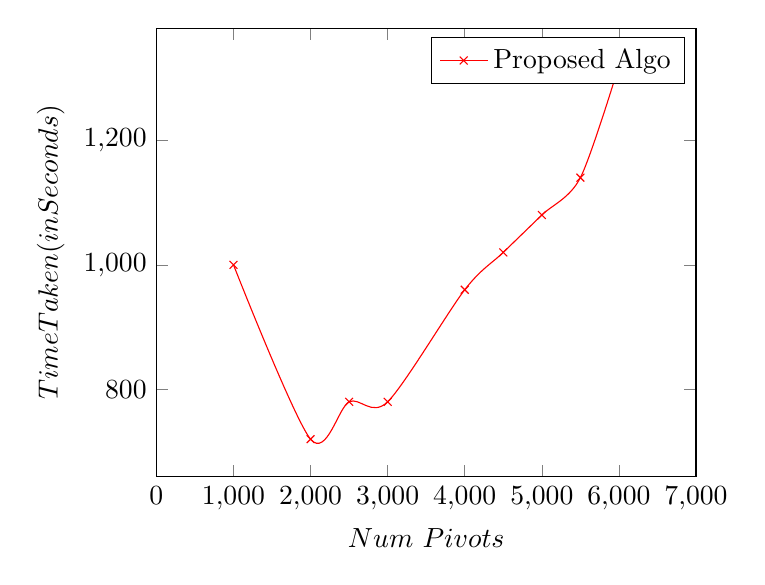
\begin{tikzpicture}[scale=1.0]
  \begin{axis}[
    xlabel=$Num\ Pivots$,
    scaled x ticks = false,
    scaled y ticks = false,
    xmin=0, xmax=7000,
    ylabel=$TimeTaken(inSeconds)$]

    \addplot[smooth,color=red,mark=x]
    plot coordinates {
      (1000, 1000)
      (2000, 720)
      (2500, 780)
      (3000, 780)
      (4000, 960)
      (4500, 1020)
      (5000, 1080)
      (5500, 1140)
      (6000, 1320)
    };
    \addlegendentry{Proposed Algo}
  \end{axis}
\end{tikzpicture}

\section{Effect of dimensions}
We evaluated the increase in dimensions and found that higher the
dimensions longer the computation time. This is because at higher dimensions the distance
between closest and farthest neighbors will be nearly same
\cite{beyer_when_1999}. This also causes increase in shuffling bytes.

\bigskip


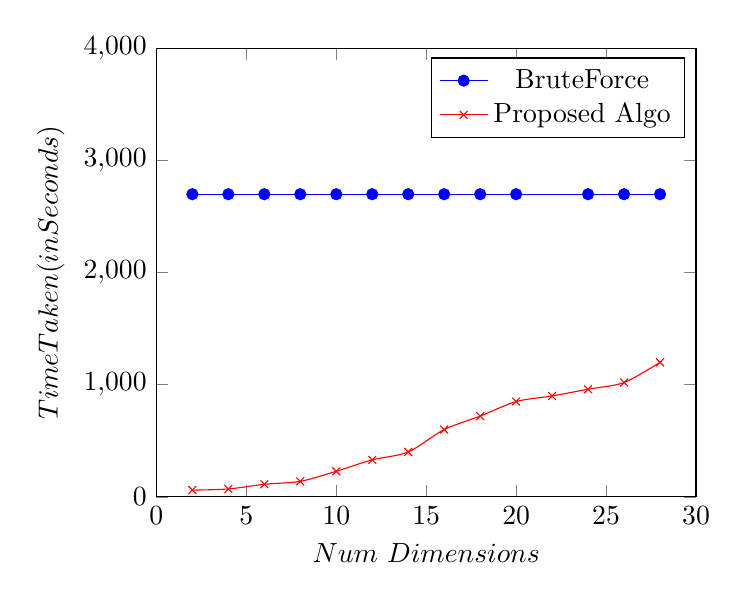
\begin{tikzpicture}[scale=1.0]
  \begin{axis}[
    xlabel=$Num\ Dimensions$,
    scaled x ticks = false,
    scaled y ticks = false,
    xmin=0, xmax=30,
    ymin=0, ymax=4000,
    ylabel=$TimeTaken(inSeconds)$]
    \addplot[smooth,mark=*,blue] plot coordinates {
      (2, 2700)
      (4, 2700)
      (6, 2700)
      (8, 2700)
      (10, 2700)
      (12, 2700)
      (14, 2700)
      (16, 2700)
      (18, 2700)
      (20, 2700)
      (24, 2700)
      (26, 2700)
      (28, 2700)
    };
    \addlegendentry{BruteForce}

    \addplot[smooth,color=red,mark=x]
    plot coordinates {
      (2, 60)
      (4, 70)
      (6, 112)
      (8, 138)
      (10, 228)
      (12, 330)
      (14, 400)
      (16, 600)
      (18, 720)
      (20, 850)
      (22, 900)
      (24, 960)
      (26, 1020)
      (28, 1200)
    };
    \addlegendentry{Proposed Algo}
  \end{axis}
\end{tikzpicture}

\section{Effect of number of nodes}
Using distributed framework should help us achieve near linear
scalability. But once we reach a threshold the perfomance start to
remain constant because many nodes will not be used fully


\medskip

\begin{tikzpicture}[scale=1.0]
  \begin{axis}[black,
    axis y line*=left,
    xlabel=Num Servers,
    ylabel=time in seconds,
    ]
    \addplot[smooth,color=black,mark=x]
    plot coordinates {
      (1, 1380)
      (2, 720)
      (3, 498)
      (4, 396)
      (5, 312)
      (6, 268)
      (7, 234)
      (8, 216)
      (9, 204)
      (10, 192)
    };
  \end{axis}

  % \begin{axis}[blue,
  %   xlabel=Num Servers,
  %   ylabel=Shuffle MBytes,
  %   axis y line*=right,
  %   axis x line=none, ]
  %   \addplot[smooth,color=blue,mark=x]
  %   plot coordinates {
  %     (1, 0)
  %     (2, 200)
  %     (3, 300)
  %     (4, 400)
  %     (5, 450)
  %     (6, 450)
  %     (7, 450)
  %     (8, 450)
  %   };
  % \end{axis}
\end{tikzpicture}

\bigskip
